\documentclass[11pt]{article}
\usepackage{geometry} % see geometry.pdf on how to lay out the page. There's lots.
\usepackage{hyperref}
\usepackage{graphicx}
\usepackage{gensymb}
\usepackage[affil-it]{authblk}
\usepackage[toc,page]{appendix}
\usepackage{pifont}
\usepackage{amsmath}
\usepackage{amssymb}
\usepackage{relsize}
\usepackage{draftwatermark}
\usepackage[mathscr]{eucal}
\usepackage{amsmath, amssymb, graphics, setspace}
\usepackage{amsthm}
\usepackage[english]{babel}
 
\newcommand{\mathsym}[1]{{}}
\newcommand{\unicode}[1]{{}}

\newtheorem{exercise}{Exercise}
\newtheorem{theorem}{Theorem}
\newtheorem{corollary}{Corollary}

\SetWatermarkText{DRAFT}
\SetWatermarkScale{6}
\SetWatermarkLightness{0.95}

\DeclareMathOperator{\atantwo}{atan2}
\DeclareMathOperator{\sign}{sign}
\DeclareMathOperator{\sense}{sense}

% \geometry{letter} % or letter or a5paper or ... etc
% \geometry{landscape} % rotated page geometry

% See the ``Article customise'' template for come common customisations

\title{Formulae for the Helix Formed by Stacking Similar Objects}
\author{Robert L. Read
  \thanks{read.robert@gmail.com}
}
\affil{Founder, Public Invention, an educational non-profit.}

\date{\today}

%%% BEGIN DOCUMENT
\begin{document}

\maketitle

%% \tableofcontents

\section{Introduction}

During the Public Invention Mathathon of 2018, software was created to view tetrahedra joined face-to-face in chains. It
was noted by the participants that when the rules for which face to add the next tetrahedron to were periodic, the resulting
chain was always a helix or a torus. A torus is a degenerate helix.

After some relfeciton, it became clear that any stack of objects of the same length joined at the same angles to each other repetitively form a helix. 
A specific example is a face-to-face connection of physical objects of the same length where the angles of the two joining
faces relative to each other control the angle and rotation of the axis at each joint. We have not yet found this simple idea articulated elsewhere. The purpose of this paper is to prove and to provide formulae for the resulting helix.

In engineering, sometimes the term ``special helix'' is use for helical curves on non-cylindrical surfaces. This paper use the term ``helix'' only in the sense of ``cylindrical helix''.
\url{https://link.springer.com/chapter/10.1007/978-94-007-2169-2_95}

\section{A Warm-up: 2Dimensions}

Considering the problem in two dimensions may be a valuable introduction.
Suppose that we consider a polygon that that as two edges, called $A$ and $B$, and that we define the length $L$ of the
polygon as the distance between the midpoints of these edges. Suppose that we are only allowed to join these
polygons by aligning $A$ of one polygon to $B$ of another polygon, with their midpoints coincident. Let us
further assume that we disallow inversions of the polygon.  Let us imagine that we have a
countable number of polygons $P_i$ indexed from $0$. Then what shapes can we make by chaining these
polygons together?

Each joint $J_i$ between polygons $P_i$ and $P_{i+1}$ will place the axes of at the same angle, $\theta$, since
our polygons do not change shape. Let us define $\theta$ to be positive
if we move anti-clockwise from $P_i$ to $P_{i+1}$ and negative if we move clockwise. 
If $\theta = 0$, the joints will be collinear.

\begin{figure}
     \centering
     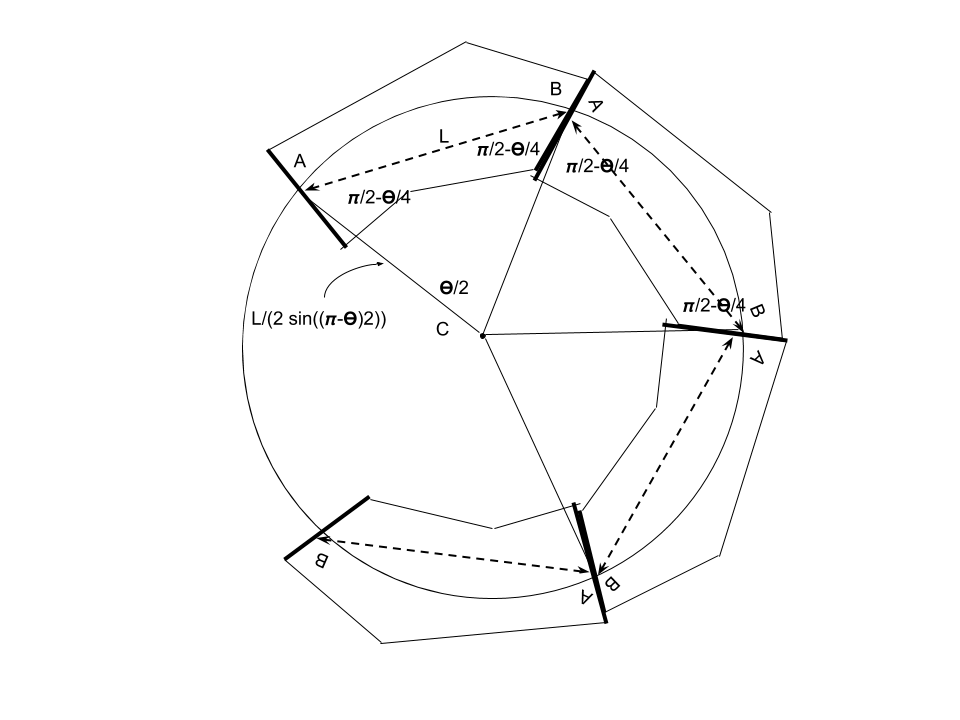
\includegraphics[width=0.80\textwidth]{figures/2DPolygonStacking.png}
     \caption{The rotatable prism of three objects}
  \label{fig:prismdiagram}
\end{figure}

If $\theta \neq 0$, it seems they polygon joints will always lie on a circle. A proof of this
is that each polygon has associated with it an isoceles triangle $A,B,C$, where $\angle CBA = \angle CAB = \theta/2$,
and $\angle ACB = (\pi - \theta)$. $AC$ and $BC$ are not necessarily aligned with an edge of the polygon.
The length $AB$ is $L$, and the lengths $AC$ and $BC$ are
$(L/2) / \sin{(\pi - \theta)/2}$. In any chain of polygons, these triangles all meet at point $C$, and there all
joints are on the circle centered at $C$ with radius $\frac{L}{2 \sin{\frac{\theta}{2}}}$.

An analogous, though far more complicated, result holds in three dimensions.

\label{sec:2d}
\section{The Discrete Helix}

In this section we consider discrete helix, or a helix evaluated only at regular points. Drawing lines between these
points create 3D polygon.

Following the Wikipedia artilce \url{https://en.wikipedia.org/wiki/Helix}, we set up a helix parametrically.
\begin{align*}
    P_x(t) &= r \sin{t}  \\
    P_y(t) &= r \cos{t} \\
   P_z(t) &= b t
\end{align*}
Such a helix has a radius of $r$ and slope (if $r \neq 0$) of $b/r$,. Note that a helix may be degenerate in two ways.
If $r = 0$, these equations become a line. If $b = 0$, these equations describe a circle in the $xy$-plane.
If $r = 0$ and $b = 0$, the figure is a point.

Such helixes are continuous, but we are investigating stacks of discrete objects. We in fact wish to derive
the parameters for a continuous helix from such discrete objects which constrain discrete points, so we wish
to study a helix evaluated at integral points. We call such an object a {\em discrete helix} or {\em delix (DEE-lix).}.
A discrete helix may be thought of as function that given an integer gives back a point in three space.
\begin{align*}
    P_x(n) &= r \sin{n \theta}  \\
    P_y(n) &= r \cos{n \theta} \\
   P_z(n) &= n d
\end{align*}

$d$ is the distance along the $z$-axis between adjacent joints, and $\theta$ is the rotation around the $z$-axis between adjacent points. $r$ is the radius of the delix. If we think of the delix as describing a polyline in 3-space, we would like to investgiate
the properties of that polyline.

\begin{itemize}
\item $L$ is the distance between any two adjacent points.
\item $c$ is the length of a chord formed by the projection of the segment between two points into the $xy$-plane.
\item $\phi$ is the angle in the plane containing two joints which is perpendicular to $xy$-plane
  (in other words the plane parallel to the $z$ axis containing two points.)
  \end{itemize}
These quantities are related:
\begin{align}
    c &= 2r\sin{\frac{\theta}{2}} \\
    L^2 &= c^2+d^2  \\
    \arctan{\frac{c}{d}}  &= \phi 
\end{align}

Now we are attempting to relate these properties to properties intrinsic to the joint or interface between
two segments or objects in the delix. If given an object, the length between the joint points $L$ is
easily measured.

\section{The Intrinsic Properties of Stacking Objects}

There seem to be two different approaches to defining the stacking of objects: the point-method,
and the angle-method.

In the point method we begin with the position of up to four joints in Cartesian space, and
seek to disover the delix which fits them.

By using the the basic fact that the points nearest each other on the skew lines drawn between a point and the midpoint between its two
adjacent points intersect the axis of the helix and are easily computed, it is relatively easy to compute $r,d,\theta$ from four points.

\begin{figure}
     \centering
     \includegraphics[width=0.80\textwidth]{figures/ObjectForStackingSetup.png}
     \caption{The rotatable prism of three objects}
  \label{fig:intrinsicdiagram}
\end{figure}

In the angle method, we start with intrinsic properties of an object, and additionally the
rule for how objects are laid face-to-face. That is, knowing the length between two
joint points and a vector normal to the faces of the two joints, we almost have
enough to determine the unique stacking of objects. The final piece is that we must
know the {\em twist}. That is, when face $A$ of a second objects is placed on face $B$
of a first object so that they are flush (that is, their normals are in opposite directions),
it remains the case that the second object can be rotated about the normals. To
define the joining rule, we must attach an {\em up vector} to each object. Then a joining
rule is ``place the second object against the first, joint point conincident to joint point,
and twist it so that its up vector differs by $\tau$ degrees from the up vector of the first
object.''

It seems clear that either method gives us everything we want to know and is computable
from the other. In the realm of comptuer graphics, obtaining four points is probably easy.
In the real of chemistry or molecular biology, where the objects are in fact molecules,
it might be easier to predict the intrinsic properties of the object and the joint twist
than to actually construct a three-object stack and measure it, so we consider the angle
method more basic.

The angle method requires:
\begin{itemize}
\item An object with two identified faces, labeled $F_A$ and $F_b$. These faces are in
  fact planes, with normal vectors $N_A$ and $N_B$. We assume that normals point out
  of the object rather than in.
\item The length $L$ of an object, measured from joint point $A$ to joint point $B$.
\item A joint twist $\tau$ defining the change in computed up-vector between objects,
  mesured at the joint face.
\end{itemize}

From the normals, we can compute an {\em up vector} which is intrinsic to the object.
We could think of the up vector as a fine mark made on each face in the same direction
(if projected onto a plane perpendicular to the axis.) When face $F_A$ of object $N+1$
is placed against $F_B$ of object $N$, object $N+1$ is twisted until the mark on $F_A$ angles
$\tau$ away from the mark on object $N$, measured anticlockwise looking from $A$ to $B$ on
object $N$.

To define the up vector, place the object so that joint $B$ is at the origin and the
axis is aligned with the $z$-axis, with the point $A$ on the negative $z$-axis.
The projection of the face normals form a minimum angle less than or equal to $\pi$
radians. Rotate the object about the $z$-axis so that the projections of the face normals
form equal angles with the negative $y$-axis. Then define the direction straight up
the $y$ axis to be the up vector. If we had a physical object, we might mark the face
normals with an arrow to mark the up vectors.

If one of the face normals is aligned with object axis, the up-vector is the opposite
of the other face normal. (If both face normals are aligned with the axis of the object,
then delix has zero radius and $d = L$, so we need do no further math.)

Mathematically, we will treat the up vector as unit-vector.
\begin{align}
  M &= \frac{A+B}{2} \\
  X &= \frac{(A+F_a) + (B+F_b)}{2} \\
  U &= \frac{M - X}{\Vert M - X \Vert}
\end{align}

The up vector is not defined when the face norms point in precisely opposite directions,
in which case $d = L$.

In the placement of the first object described above, it would
be nice to know where the position of point $B$ on the second
object is. This can be obtained by computing the Euler angles
of the face normal $N_A$ at the origin, and then simply
adding the negation of the Euler angles $N_B$, and using
the resulting angles to compute a rotation $R(N_A,N_B)$ to be a applied to
a vector of length $L$, and then performing the twist by $T(\tau)$. This process can be repeated at
the point $B_1$ (though no longer at the axis) to generate
four or more points. In fact the entire process of constructing
the stack could be thought of a series of ``rotate then translate'' steps by the composition of the rotation matrixes $RT$ applied to a vector $\overline{AB}$ and the up vector.
However, it is a tiny bit of work to compute this given only
the intrinsic properties of the object and joint.

Note: we have shown we can compute from 4 points.
More elegant however, would be to construct a similar
construction using the axis-intersecting lines without
computing 4 points, perhaps from a pure geometry in some way.

TODO: Actually giving the transformation matrix here would be nice.
How would we test? 

TODO: Compute the vector angle between axes here. In this positioning, compute where
point B of the second object will be.

Note: The twist is not the same as $\theta$. When $\tau = 0$, $\theta = \alpha$,
I think. Possible $\theta = \alpha + $ some function of $\tau$.

Note: Possibly theta goes down as tau goes up.

Note: Considering the pitch of the discrete helix may be useful
in relating variables.

Note: I now think we can think in terms of the skew lines (the
joint lines), and I believe $\tau$ is directly the angle
formed with the up vector, that the up-vector aims at
the mid point of the axis between the intersection skew line
points, and that angle bend $\alpha$ (or $(\pi - alpha)/2$)
let's us determine the skew line as well.  So we have
the mid point, and we have another line based purely
on $\tau$ and $\alpha$, so that may allow $\theta$
to be computed more simply than the skew line intersection
construction.

Todo: Try to do my 4-point solution with an Midpoint and
upvector solution.

Todo: Try to prove that $\tau$ is really either the
angle bisector angle or twice it.

Todo: Create a definition of the ``sidedness'' of delix,
in terms of the number of sides in one pitch, and relate
this matehmatically to the other points.


\section{Computation of Discrete Helix}

In this section we attempt to derive formulae for $r,d,/theta$ from
the instrinsic properties of the object.

\section{Old Work}

The most easily measured relationship between the segments
is the angle $\alpha$ in the plane containing both of the segments. (If the segments are coincident and therefore
parallel $\alpha$ will be $\pi$. If $\alpha < \pi/2$, the segment ``bends backward''.
The final measure that is needed is the rotation about a member between the elements attached to it.
Let us call this angle $\psi$. That is, if you look along the axis of an object at the line
between the joints, the two members form an angle between 0 and $\pi /2$. 

\begin{align*}
    A &= P(-1)  \\
    B &= P(0) \\
    C &= P(1)
\end{align*}

$A,B,C$ form an isoceles triangle that contains $\overline{AB}$ and $\overline{BC}$, and therefore the angle $\alpha$ is in
this plane. Forming the kite $ABCO$, we see that one diagonal is $r$ and the other diagonal is $2 r \sin{\theta}$, where
$y = r \sin{\theta}$ is half of this diagonal. 

\begin{align*}
    y &= r \sin{\theta}  \\
    z^2 &= c^2 - y^2 \\
    z^2 &= c^2 - (r \sin{\theta})^2 \\    
    q^2 + z^2 &= L^2 \\
    q &= \sqrt{L^2 - z^2} \\
    q &= \sqrt{L^2 - (c^2- (r\sin{\theta})^2)} \\
    q &= \sqrt{L^2 + (r\sin{\theta})^2 - (2r\sin{\theta/2})^2 } \\        
    \sin{\alpha/2} &= q/L \\
    q &= L \sin{\alpha/2} \\
    \alpha/2 &= \arcsin{q/L} \\
    \alpha &= 2 \arcsin{\frac{\sqrt{L^2 + (r\sin{\theta})^2 -
          (2r\sin{\theta/2})^2}}
      {L}} \\ 
\end{align*}

Note $y$ is in the projected kite, $q$ is in the slanted kite.
Rearranging these relationships in terms of known quantites $L, \alpha, \psi$, we have:

\begin{align*}
  \sin{\alpha/2} &= q/L \\
  q &= L \sin{\alpha/2} \\    
  z^2 &= L^2 - q^2 \\
  %% Now we must use \psi
  \beta &= \frac{\pi - \theta}{2} \\
  \frac{z}{c} &= \cos{\beta} \\
  c &= \frac{z}{\cos{\beta}} \\
  y^2 &= c^2 - z^2 \\
  r &= \frac{y}{\sin{\theta}} \\
  d^2 &= L^2 - c^2 \\
  \phi &= \arctan{c/d} \\
\end{align*}

I think we can compute $\psi$ from $\theta$ easily enough. The problem is going the other way.

\subsection{An alternate approach}

Rather than starting with $\alpha$ and $\psi$ as inputs, we can think of a vector $v$ that
moves in the positive $\overline Z$ direction, $\overline Z = \overline P_1 - \overline P_0$, and
the angle $\theta$ which $Z$ rotates about the $z$-axis at each step. If a rotation matrix $M$
represents rotation about and $T$ represents translation along the $z$-axis, then $P_n = (M+T)^nP_n$.


\section{Three dimensions}

\subsection{New Approach}

We want to compute everything from properties intrinsic to the object and the joint process.
These are the length, the face normal vectors, and the joint twist. These are the
inputs to our process.  From this we can compute several joints by:
1) Placing the object joint-to-joint aligned along their axes;
2) Computing from the face angles the rotation that makes the normal to B the
negative of the normal to A, that is, the rotation that moves A into -B.
3) Apply this rotation around the joint.
4) Rotate along the axis until the up vectors match.

The ``Up vectors'' are computed to be in the line between the midpoints of points
pointed to by the face normals, and the mid point of the axis, projected to be normal
to that axis.

Using this intrinsic method, we can get as many points as we need of the stacked objects.

From these intrinsic property, the vector angle between axes of different objects
is determined.

From these points, we can easily compute a ``tilt and twist'' approach, which defines
$\alpha$ as the tilt and $\psi$ as the twist. Those two parameters now become
an output of this process above.  Not the ``twist'' is measured IN THE PLANE OF
FACES.

The remaining task is to find an $(r,\theta)$ helix representation that gives us
what we need.

Conjecture: the twist is the same (or at least monotone in) as $\theta$.

Proof Sketch: Imagine moving so many times around the helix that
our $(x,y)$ coordinates are similar to your starting point. The up vector
for this object must point in approximately the same direction as the up axis
you started with, by symmetry. If $\theta$ is anything other an integral
factor of the twist, this would be impossible.

Alternative: The up vector at the midpoint of the object must aim at the
axis of the helix. This must always be true. Therefore, the 

TODO: We are still fundamentally seeking $r,\theta$ from these specifications.
A formula for that is of the utmost importance.

Note: If the up vectors intersect the axis of the helix, we can find two
points on this line using the wikipedia article: \url{https://en.wikipedia.org/wiki/Skew_lines}
and the distance between these two points. This will allow us to find $r$, I think.

Using the method from skewlines to find two nearest points, we can then solve for
the distance between this line and $A$ or $B$ and we have $r$.

So, the way to test this is to generate a helix. Use the helix to generate
the midpoints and up vectors. Then at least check that we can back out and
obtain our same radius and theta for the delix.  Then the problem becomes the
computation of the points and up vectors from the intrinsic properties of the block,
which I believe to be possible.  Which should I attack first?

Let us first prove that given 3 points and two up vectors we can recover the helix.

When we have a Mathematica procedure for that, then we can generate these inputs
from the object inputs of $L,\overline{A},\overline{B}$,and twist.

Is twist the same as theta? No, it is not---but they are related by $/phi$.



\subsection{Old Approach}


Consider a slender cylinder or prism with two faces $F_0,F_1$ cut at arbitrary angles to the axis of the cylinder.
Joining two such cylinders at the axes by placing $F_0$ angainst $F_1$ produced a joint with a difference in
angle between the axes of $\alpha$ and a rotation of the orienation of the faces about the axis of $\theta$.
Note that $\alpha$ and $\theta$ are a function of the vectors normal to the faces to be joined, but are not the same as them. $\alpha$ and $\theta$ are likely combinations of the face angles.

\begin{theorem}[Stacking Helix]
  The joints of a sequential stack of objects of length $L$ whose joints axis change by $\alpha$ and orientation rotate
  by $\theta$ are intersected by a helix of radius and pitch easily numerically computable
  from  $L,\alpha$, and $\theta$.
\end{theorem}

\begin{figure}
     \centering
     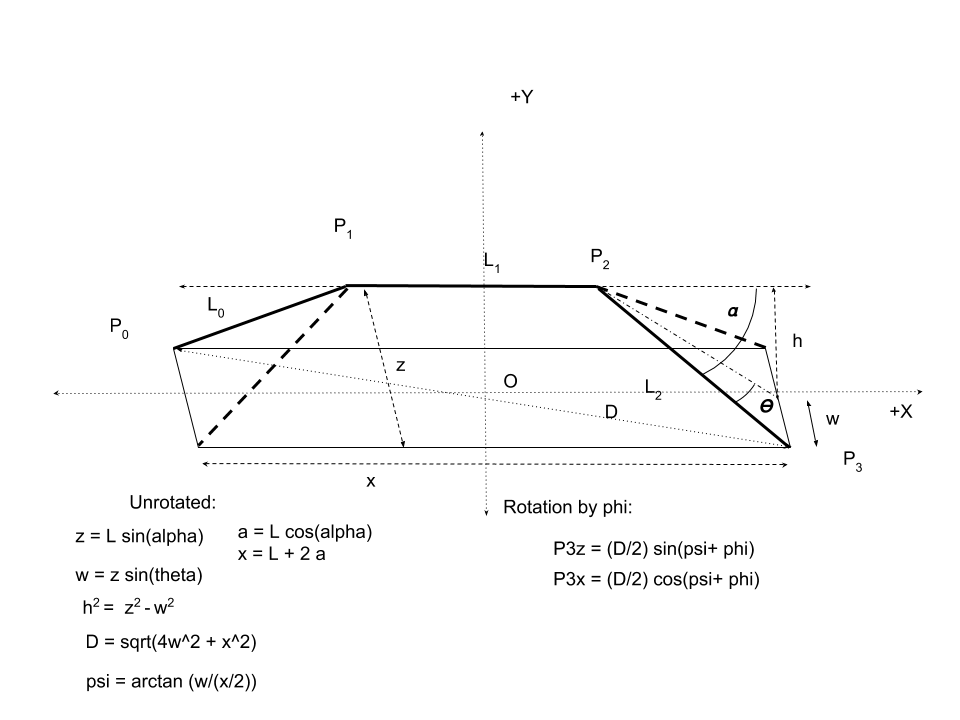
\includegraphics[width=0.95\textwidth]{figures/StackedSetup.png}
     \caption{The rotatable prism of three objects}
  \label{fig:prismdiagram}
\end{figure}

\begin{proof}

  In Figure \href{fig:prismdiagram}, let $L_i$ be the $i$th instance of the length-$L$ objects. Let $\alpha$ be the
  change in angle in the axes at a joint (the point were axes meet) measured in the plane containing the axes of both objects. (If these axes are parallel (and therefore coincident) define $\alpha$ to be 0.
  Let $\theta$ be the change in orientation relative to the axis,
  or, the half-angle formed by $L_0$ and $L_2$ when projected onto a plane normal to the axis of $L_1$.
  Without loss of generality, choose the measures of these angles in radians so that
  $0 \leq \theta < \pi/2$ and $0 \leq \alpha < \pi$.
  Take $\alpha < 0$ to mean that objects $L_0$ and $L_1$ bend away from each other,
  and $\alpha > 0$ to mean that the objects $L_0$ and $L_1$ bend toward each other.

  If $\theta = 0$ and $\alpha > 0$, the stack will form a circle-like structure or radius 
  $\frac{L}{2 \sin{\frac{\alpha}{2}}}$, as shown in Section \ref{sec:2d}, where as if
  $\theta = 0$ and $\alpha < 0$, then stack will form a sawtooth-like structure.

  Note that any angle $\alpha$ is possible, if we do not concern oursleves with the self-collision
  of physical objects. $\alpha > \pi/2$ means the stack ``turns back on itself'' to some extent.

  If we arrange object $L_1$ so that its axis lies on the $x$-axis and its midpoint is at the origin,
  $L_0$ and $L_1$ extend from it symmetrically in the projection onto the $yz$-plane along the $x$-axis, which is always possible, and define $h$ to be the height of the faces of $L_0$ and $L_2$ along the $y$-axis
  and $w$ to be the distances between these faces in the $z$-dimesnion. Then we have:

  \begin{align*}
z &= L \sin{\alpha} \\
w &= z \sin{\theta} \\
h &= \sqrt{z^2 - w^2} \\
  \end{align*}

  Now we seek the formula for the helix which intersects the joints. To find the radius of this helix,
  we conceptually place our three objects in a cylinder, with the axis of $L_1$ along the surface
  of the cylinder aligned with the axis. We can size this cylinder to include the joints at the
  extreme ends of $L_2$ and $L_0$ as well. However, the $L_1$ axis lies on the surface, but
  the axes of $L_0$ and $L_2$ in general do not. If there exists a helix which intersects all
  joints, all axes will cut through this cylinder in the same way, creating chords in the projection
  into the $yz$-plane of the same length. Name these chords $c_0,c_1, and c_2$.

  Because we will need them later, we work out the geometry of this prism-like stack of three
  objects completely.
  \begin{itemize}
  \item The three objects are named $L_0,L_1,$ and $L_2$.
    $L_0$ has joints $P_0$ and $P_1$,
    $L_1$ has joints $P_1$ and $P_2$,
    $L_2$ has joints $P_2$ and $P_3$.
  \item  $x$ is the total length of the prism along the $x$-axis.
  \item $z$ is the length of the ``face'' of the prism, and the length
    of the chord before any rotation $\phi$ about the $y$-axis.
  \item $w$ is half of the width of the prism in the $z$-dimension.
  \item $h$ is the height of the prism in the $y$-dimension.
  \item $D$ is the length of the diagonal from $P_0$ to $P_3$.
  \item $\psi$ is the angle of $\overline{P_0P_3}, \arctan{(w/(x/2))}$.
    \item $\phi$ is the amount we will have to rotate the prism about the $y$-axis.
    \end{itemize}
Given these defintions about our assumptions, the cord lengths are:
\begin{align*}
  \psi &= \arctan{(w/(x/2))} \\
D &= \sqrt{4w^2+x^2} \\
c_1 &= L \sin{\phi} \\
c_2 &= \sqrt{h^2 + ((1/2)(D\sin{(\psi+\phi)}-L\sin{\phi})^2}  \\
c_0 &= c_2 \\
  \end{align*}
  

  We can imagine turing our 3-object stack and simulataneously increasing the size of our intersecting
  cyliner. If we turn the stack about the $y$-axis by $\phi$ degrees and keep the cylinder intersection
  the two faces of $L_1$, then the length of the $L_1$ chord will gradually increase. At the same time,
  the $L_0$ and $L_2$ chords will change their length, possibly increasing or decrasing.
  When $\phi = 0$, $c_0 = z, c_1 = 0, c_2 = z$.

  Equating these quantities to find when $c_2 = c_1$, we have a trigonometric equation with
  a single unknown, $\phi$.
    \begin{align*}
      L \sin{\phi} &= \sqrt{h^2 + ((1/2)(D\sin{(\psi+\phi)}-L\sin{\phi})^2} \\
      %% To put this in the language of Wolfram Alpha....
      %% L* sin(x) = sqrt(A + ((1/2) *(D* sin(x + B) - L * sin(x)))^2)
      %% At present, Mathemtatic does not appear able to solve this.
    \end{align*}

    Although Mathematica does not appear to be able to solve this equation, it appears
    to be a smooth equation in the variable $\phi$ and we believe from the physical
    structure of the problem that will have only a single solution, so we can
    solve this numerically with a Newton-Raphson solver easily.
    
    Thus, by rotating our stack of objects $\phi$ degrees around the $y$-axis 
    all four faces of our three objects intersect a cylinder on its surface with
    equal rotational and axial distance. The axial distance between any two joints
    on the same object is $L \cos{\phi}$,
    and the length of the projected chord is $L \sin{\phi}$.

    The points $P_0,P_1,P_2,$ and $P_3$ now exist on a cylinder or unknown radius parallel
    to $x$-axis, and are evenly spaced along and evenly rotated about the axis of the
    cylinder. The joints points thus coincide with a general helix.

    Let us choose our coordinate system so that the $x$-axis corresponds to the
    axis of the helix. The general equation for the helix is:

\begin{align*}
    P_x(n) &= \kappa  t  \\
    P_y(n) &= r \cos{t} \\
   P_z(n) &= r \sin{t}
\end{align*}

We seek to discover $r$ and $\kappa$ based on our knowledge of $P_3$ and $P_2$.
In particular, we can deduce from the axial spacing there exists some $t_0$ such
that $P_2 = P(t_0)$ and $P_3 = P(3t_0)$.
Since we know that after rotation that:

  \begin{align*}
    P_{3z} &= (D/2) \sin{\phi + \psi} \\
    P_{3z} &= r\sin{3t_0} \\
    P_{2z} &= \sin{\phi} \\
    P_{2z} &= r\sin{t_0}
  \end{align*}
  We can use symbolic computation to solve this system of 2 equations and 2 unkowns:
  \begin{align*}
    r\sin{3t_0} &= (D/2) \sin{\phi + \psi} \\
    r\sin{t} &= \sin{\phi}
  \end{align*}
  Defining symbols:
  \begin{align*}
    E &= (D/2) \sin{\phi + \psi} \\
    F &= \sin{\phi}
  \end{align*}
  Wolfram alpha solves the system:
  \begin{align*}  
    r\sin{3t_0} &= E \\
    r\sin{t_0} &= F
  \end{align*}
  giving the result ($3F \neq E$ and $F \neq 0$), and ignoring multiples of $2\pi$ in $t$:

  
  \begin{align*}  
    r &= \frac{2F^{\frac{3}{2}}}{\sqrt{3F - E}} \\
    t_0 &= -2 \arctan{x}
      \frac{r +
        \sqrt{- \frac{F^2(F+E)}{E-3F}
        }
      }
           {F}
     \\
  \end{align*}
  From which, using $P_{2x} = L/2 = \kappa t_0$, we conclude:
  \begin{align*}  
    r &= \frac{2F^{\frac{3}{2}}}{\sqrt{3F - E}} \\
    \kappa &= \frac{L}{4 \arctan{\frac{r + \sqrt{- \frac{F^2(F+E)}{E-3F}}}{F}}}
  \end{align*}.
  Putting this all together we have:
  \begin{align*}
    a &= L \cos{\alpha} \\
    x &= L + 2a \\
    z &= L \sin{\alpha} \\
    w &= z \sin{\theta} \\
    h &= \sqrt{z^2 - w^2} \\
    D &= \sqrt{4w^2+x^2} \\
    \phi &= \arctan{\frac{z}{L}} \\
    E &= (D/2) \sin{\phi + \psi} \\
    F &= \sin{\phi} \\
    r &= \frac{2F^{\frac{3}{2}}}{\sqrt{3F - E}} \\
    \kappa &= \frac{L}{4 \arctan{\frac{r + \sqrt{- \frac{F^2(F+E)}{E-3F}}}{F}}}
  \end{align*}
  Using these values derived exclusively from the inputs $L,\alpha, and \theta$, we can
  evalute the formula for the general helix only and integral values of $n$ to
  obtian a formula for precise the joint points of this any such stack.
\begin{align*}
    P_x(n) &= \kappa  t0 (1 + 2n)  \\
    P_y(n) &= r \cos{t0 (1 + 2n)} \\
    P_z(n) &= r \sin{t0 (1 + 2n)}
\end{align*}

\end{proof}

\section{Checking against comprehensible values}

Unfortunately, the complexity of these formualae exceed the author's comprehension.
However, we may check these formuale by graphing them against comprehensible
examples. Obvious examples are extreme solutions, where $\alpha$  and $\theta$ are
$0$ or $\pi/2$, for example. We also have the particular non-trivial example
of the Boerdick-Coxeter tetrahelix, formed by regular tetrahedra, which has
been studied enough to have a known pitch.



\section{Implications}

One of the implcations of having a formulaic understanding of the math
is that it may be possible to design helixes
of any radius and pitch by designing periodic (possibly scalene) segments. Combined with slight
irregularites, this means that you have a basis of design molecular helices
out of ``atoms'' which correspond to our objects.

This would mean that if you wanted to build a brace of length exactly 3 meters
with bars of exactly 1/2 meter you would be able to come as close to this
as mathematically possible.






\section{Applied to Periodic Regular Simplex Chains}

\begin{corollary}
  Every regular simplex chain formed by a periodic generator has a helical structure.
  \end{corollary}

Prove or disprove that {\em every} periodic 3D Generator generates a figure contained within a cylinder of unbounded length but bounded diameter.

Note: Every example that we have tested exhibits this property. We believe it is a property of any repeated structure, not related to simplices.
However, we do not yet know the name of this theorem or principle. We conjecture that every stack of repeated truncated prisms
forms a helical aperigon, which is hinted at but not stated in the Wikipedia article\url{https://en.wikipedia.org/wiki/Skew_apeirogon}.

Note: Rob believes a proof that any periodic structure fits within a cylinder is possible, and that it should be possible to give a formulaic bound
on the diameter of this cylinder (under some assumptions.) The key to the proof is to use symmetry and focus on the the center of three
such objects, observing that the other two must necessarily bend towards or away from each other in a way describable by two angles.
A formula for the cylinder as a function of these angles would convincingly complete the proof.

Note: This paper may be critical.

\url{https://arxiv.org/pdf/1610.00280.pdf}

\url{https://www.impan.pl/wydawnictwa/preprints_impan/p741.pdf}

\url{https://math.stackexchange.com/questions/878051/why-does-a-3d-line-of-segments-with-constant-angles-always-make-a-helix/878079#878079}

\url{https://www.sciencedirect.com/science/article/pii/S0097849313001787}
\url{https://www.win.tue.nl/~wstomv/publications/mathmitering-final.pdf}
\url{https://www.clinbiomech.com/article/S0268-0033(98)00080-1/abstract}
\url{http://www.close-range.com/docs/Computing_Euler_angles_from_a_rotation_matrix.pdf}
\url{https://gist.github.com/peteristhegreat/3b76d5169d7b9fc1e333}
\url{https://link.springer.com/chapter/10.1007/978-94-007-2169-2_95}
\url{https://www.sciencedirect.com/science/article/pii/S0022309303008573}
\url{https://www.sciencedirect.com/science/article/pii/S0022309307005583}

This reference is EXTREMELY IMPORTANT
\url{https://link.springer.com/article/10.1023/A:1015863923728}
\url{https://www.researchgate.net/publication/226976531_Helical_Structures_The_Geometry_of_Protein_Helices_and_Nanotubes}
This reference clearly states that any repetitive unit gives rise to a helix, and gives some species: the icosahelix, for example, and gives a 96-tet ring (not quite regular, like this work.)  It gives a linear algebra way of talking about the transform. It does implies the helix is deducible from the transformation matrix, but does not appear to give any formular or method for describing it.

Need to get and read this:
\url{https://books.google.com/books?hl=en&lr=&id=1LZlSZ7ORrQC&oi=fnd&pg=PP1&ots=0hSEwJvlUB&sig=xNG9UWv_H1OXHwaOiOBJN7TW6xA#v=onepage&q&f=false}

This may be worth reading:
\url{https://link.springer.com/article/10.1007/PL00011063}

This is worth getting:
\url{https://books.google.com/books?hl=en&lr=&id=FHPlDWvz1bEC&oi=fnd&pg=PP1&ots=TsOnodavEZ&sig=HO86UUVlqRVWGqY-Tv02nb7x7NA#v=onepage&q&f=false}

Some discussion of ``screw transformations''
\url{http://dergipark.gov.tr/download/article-file/56483}
\url{https://ieeexplore.ieee.org/document/56653}

CRITICAL:
\url{https://ieeexplore.ieee.org/stamp/stamp.jsp?tp=&arnumber=56653}

This mentions Rodrigues's equation (p. 7)
\url{https://www.cc.gatech.edu/~hic/8803-Mobile-08/slides/1_draft.pdf}

This is a valuable reference
\url{http://www.12000.org/my_notes/screw_axis/index.htm}


\bibliographystyle{unsrt}
\bibliography{gluss}


\end{document}

The following math in Mathematica may be useful.

Note: Mathematica has build in Vector Angle function that can be used for alpha!!

(* c = 2 r Sin[theta/2] *)

Chord[r_,theta_] := 2 r Sin[theta/2]
 (* 1 == c^2 + d^2 *)
DZ[r_,theta_] := Sqrt[1 - Chord[r,theta]]
(* Note, this may be a problem --- Chord lenght can be diameter (2r), but I am treating it as 1 here *)
(* Some radiuses are not possible for some thetas with a length of one *)
(* Maximum radius as a function of theta *)
Mxr[theta_] := MaxValue[1 == 2 r Sin[theta/2],{r}]

Mxr[theta_] := 1/ (2  Sin[theta/2])


 Note: I should go ahead and make these functions....

(* P0 = {0, r, 0} *)
(* P1 = {r Sin[theta], r Cos[theta], d} *)
(* P2 = {r Sin[2 theta], r Cos[2 theta], 2 d} *)
(* P3 = { r Sin[3 theta], r Cos[3 theta], 3 d} *)
(* S0 = P0 - P1 *)
(* S1 = P1 - P2 *)
(* S2 = P2 - P3 *)
P[n_,r_,theta_] := { r Sin[n theta], r Cos[n theta], n DZ[r,theta]}
S[n_,r_,theta_] := P[n+1,r,theta] - P[n,r,theta]


AlphaC[r_,theta_] := VectorAngle[S[0,r,theta],S[1,r,theta]]


f[r_, theta_] := 
 ArcCos[-1 + (r - r Cos[theta]) (-r Cos[theta] + r Cos[2 theta]) + 
   4 r^2 Sin[theta/2]^2 - 
   r Sin[theta] (-r Sin[theta] + r Sin[2 theta])]

Plot3D[f[r, theta]/ Degree, {r, 0, 2}, {theta, -Pi/6, Pi/6}, 
 AxesLabel -> Automatic]


Plot3D[AlphaC[r, theta]/ Degree, {r,0,N[Mxr[Pi]]}, {theta, 0, Pi}, 
 AxesLabel -> Automatic]

(*

Note: Given that we can compute $\alpha$ from $r,\theta$ in this way, one interesting thing to ask
is simply what is the minimum or maximum r (or theta) that matches an alpha. The maximum r is the
largest helix that matches, the minimum is the smallest. But with $\psi$ we will know more.
*)

PlaneNormal[a_, b_] := Normalize[Cross[a, b]]
(* Maybe psi is just theta? *)

Psi[pv0_, pv1_, v_] := 
With[{n = PlaneNormal[pv0, pv1]}, ArcSin[(n.v) /(Norm[v] Norm[n])]]

(* This is computing the angle between planes
PsiC[rx_,thetax_] := 
With[{r = rx,theta = thetax}, Evaluate[Psi[S[0,r,theta],S[1,r,theta],S[2,r,theta]]]]


Plot3D[PsiC[r, theta]/ Degree, {r, 0, N[Mxr[Pi/2]]}, {theta, 0, Pi/2}, 
 AxesLabel -> Automatic]

(*
Note: A strategy for computation is: given alpha, find maximum or minimum radius.
Then slow change radius until \psi if find.  However, Mathematic has optimization
built in, so we may be able to use an energy function.
*)

Enrg[alpha_,psi_,r_,theta_] := (AlphaC[r,theta] - alpha)^2 + (PsiC[r,theta] - psi)^2


(* These seem to work, but they produce rules, instead of values, what up with that? *)

Rx[alpha_,psi_] := r /. FindMinimum[Enrg[alpha,psi,r,t],{r,t}][[2]][[1]]
Tx[alpha_,psi_] := t /.  FindMinimum[Enrg[alpha,psi,r,t],{r,t}][[2]][[2]]

(* This should return 2! *)
(* Is Psi the VectorAngle of the Normals of each ABC joint? *)
Rx[AlphaC[2, Pi/20], PsiC[2, Pi/20]]
FindMinimum[Enrg[AlphaC[2, Pi/20], PsiC[2, Pi/20],r,t],{r,t}]

Unprotect[$PerformanceGoal]
$PerformanceGoal = ``Speed''

Plot3D[Rx[a,p]/Degree, {a,0,Pi/10},{p,0,Pi/10}]

(* Now that we can in theory find Rx, Tx as a function of alpha and psi,
It is important that we have a check function (or two.)
The best check would be to use a reconstruction based on transformations
of alpha and psi. I need to think about how this should be done with a
RollPitchYaw Matrix, and in what order. First you by \alpha, then you rotate by \psi.
I think we are doing ``Pitch, Roll, Yaw''. First we Pitch by \alpha, then
we Roll into the plane of the joint, then we yaw by \psi.
In fact what we are trying to do is to fly a little airplane in a helical course.
``Pitch down by alpha'', ``Yaw by psi'', ``roll so that we are perpendicular
to the the plane of the last joint''.  Maybe we never need to the roll component.
I want intrinsic angle rotation (by the definition.) We do seem to have a mobile
frame of reference.
So in fact I want EulerMatrices, not RollPitchYaw matrices.

Euluer[{\alpha,\beta,\gamma},{a,b,c}], where a,b,c = 1,2,3, let us specify those.
So we need to define how our mobile frame works. We will want $y$ to always point
``out'' of the helix, ``z'' to point along the motion'', and $x$ to be
tangential to the helix.

If we start with the intrinsic frame aligned with the extrinsic frame, repeated
transofrmations will produce a helix, but not about the $z$ axis.
We have so far described our mostion as ``rotate about y'' by $\alpha$, then
rotation about $x by $\psi$. Then our $z$ axis would be pointed in the
write direction, we would translate  by $z$, in the intrinsic frame of refrence,
and repeat.

Note, mathematica seems to have a way to render a helix, this would be very useful to me:
*)

ListPointPlot3D[
Table[Table[{t, Cos[t + s Pi/2], Sin[t + s Pi/2]}, {t, 0, 
      5 Pi, .2}], {s, 4}], BoxRatios -> Automatic]

Graphics3D[
GeometricTransformation[{Hue[#/Pi], Sphere[{5, 0, 0}, 1]}, 
  EulerMatrix[{#, Pi/2, #}]] & /@ Range[0, 2 Pi, Pi/16]]

(* My claim is that we can somehow combine an EulerTransformation with a translation
to end up with a helix.

We can call GeometricTransoforamtion on an Euler matrix, can we pass a vector
as an object? Can we create an object of length L which is a vector
and then create a transformation?
*)

Graphics3D[Arrow[{{1, 1, 1}, {1, -1, 2}}], Axes -> True, 
  AxesLabel -> {"X", "Y", "Z"}, ImageSize -> Large]

Graphics3D[
GeometricTransformation[{Hue[#/Pi],Arrow[{{1, 1, 1}, {1, -1, 2}}] }, 
Composition @@ {
     TranslationTransform[{1, 1, 1}],
      EulerMatrix[{0, Pi/2, #}]
}] & /@ Range[0, 2 Pi, Pi/16]]


 EulerMatrix[{Pi/15, Pi/20, 0}] [1,1,1]


 myt = TranslationTransform[{0, 0, 1}] EulerMatrix[{Pi/15, Pi/20, 0}]


 Graphics3D[{
  Opacity[1]
  , Red
  , Arrow[{{0, 0, 0}, {1, 0, 0}}]
  , Green
  , Arrow[{{0, 0, 0}, {0, 1, 0}}]
  , Blue
  , Arrow[{{0, 0, 0}, {0, 0, 1}}]
  , Opacity[0.2]
  , GeometricTransformation[Cuboid[-{1, 1, 1}/4, {1, 1, 1}/4],
   Composition @@ {
     RotationTransform[Pi/4, {0, 0, 1}]
     , TranslationTransform[{1, 1, 1}]
     }
   ]
 }]
 
 Graphics3D[{
  Opacity[1]
  , Red
  , Arrow[{{0, 0, 0}, {1, 0, 0}}]
  , Green
  , Arrow[{{0, 0, 0}, {0, 1, 0}}]
  , Blue
  , Arrow[{{0, 0, 0}, {0, 0, 1}}]
  , Opacity[0.2]
  , GeometricTransformation[Cuboid[-{1, 1, 1}/4, {1, 1, 1}/4],
    Composition @@ {
       RotationTransform[Pi/15,{0,1,2}],
     , TranslationTransform[{1, 1, 1}]
     }
   ]  & /@ Range[0, 5, 1]
 }]


 Graphics3D[
   GeometricTransformation[{Hue[#/Pi],Arrow[{{1, 1, 1}, {1, -1, 2}}] },
       Composition @@ {
       RotationTransform[Pi/15,{0,1,2}],
     , TranslationTransform[{1, 1, 1}]
     }
 ]]


 Composition @@ {
     RotationTransform[Pi/4, {0, 0, 1}]
     , TranslationTransform[{1, 1, 1}]
 }

 Graphics3D[
   
  (GeometricTransformation[Cuboid[-{1, 1, 1}/4, {1, 1, 1}/4], 
   Composition @@ {RotationTransform[Pi/4, {0, 0, #}], 
     TranslationTransform[{1, 1, #}]}]) & Range[3]

 ]

double[x_] := 2 x
 
Nest[double,#,4] & Range[3]

(* Now, what we really want to do here, is  construct
a transform out of \alpha, \pi, ending up with the arrows head to tail
*)

Clear[ComposeN]
ComposeN[0] = ScalingTransform[{1,1,1}]
ComposeN[1] = Composition @@ {
  RotationTransform[ Pi/6, {0, 1, 0}],
  Composition @@ {
    TranslationTransform[{1, 1, 1}],
    RotationTransform[ Pi/6, {0, 0, 1}]
  }
}

ComposeN[n_] :=  Composition[ComposeN[Floor[n/2]],ComposeN[Ceiling[n/2]]]


 myarrows = 
 Table[
   GeometricTransformation[{
     Arrow[{{0, 0, 0}, {0, 0, 2}}],
     Arrow[{{0, 0, 0}, {0,1/2, 0}}]},   
     ComposeN[i]
   ],{i,1,10}
   ] 
 
 Graphics3D[myarrows]


 (* I think to do what I want, I need to do my own transformationns. *)
 (* An object is a vector and an upvector.
 The 0th object is a z-aligned vector starting at the origin, with a y upvector.
 The n+1th object is:
 A) Take the nth object (AB), find the head B of the vector.
 B) Create a vector of length N pointing in the same direction as the nth object.
 C) Translate it along the nth object to the head.
 D) Relative to 
 E) Rotate it in the AB coordinate frame in the Y direction by Alpha.
 F) Rotate it in the X direction by Psi.
 G) Apply these same arguments to the up Vector.

 Note that Mathematica has powerful RotationMatrix functions built in to which
 we can use the Nth vectors as input, to rotate in a plane. So in this sense
 we may actually be able to accomplish this.
*)

(* I'm going to try to use F to mean the nth object. *)
(* We will make the first to points computed from the Helix *)
F[0,alpha_,psi_,init_] := init

(* We are forced to pass the initial object in as a starting point *)
F[n_,alpha_,psi_,init_] :=
  With[{Prev = F[n-1,alpha,psi,init]},
      With[{
          A = Part[Prev,1], B = Part[Prev,2], U = Part[Prev,3]},
        With[{BA = B-A, UA = U-A},
        (* now we want to contruct the parts of P_n *)
        Module[{NA,NB,NU,RA,RP,NV},
          NA = B;
          V = BA;
          (* This is in theory spanned by BA, UA *)
          RA = RotationMatrix[alpha,{BA,UA}];
          RP = RotationMatrix[psi,BA];
          NB = RP.RA.V;
          NU = RP.RA.UA;
          NB = NB + B;
          NU = NU + B;
          {NA,NB,NU}
    ]
  ]]]]

  
  (* F requires an initial object (of three points, A, B Up.) These
  are essentially P[0],P[1], and P[0] + [0,1,0]. *)

  FTest[n_,alpha_,psi_,r_,theta_] :=
  With[{P0 = P[0,r,theta]},
    Part[F[n,alpha,psi,{P0,P[1,r,theta],P0+{0,1,0}}
      ],1]
    - P[n,r,theta]]
    
  FTest[1,Pi/8,0,1,0]

  FStratTest[k_,alpha_,psi_] :=
  With[
    {r = Rx[alpha,psi], t = Tx[alpha,psi], P0 = {0,0,0} },
    With[{P0 = P[0,r,t], P1 = P[1,r,t]},
      With[{init = {P0,P1,P0+{0,1,0}}},
    Print["alpha, psi, r, t ",alpha,", ",psi,", ",r,", ",t 180 / Pi];    
    For[i = 0, i < k, i++,
      Print["point ",i];
      Print["P ",P[i,r,t]];
      Print["F ",Part[F[i,r,t,init],1]]
      ]
    ]
  ]]

  (* Pretty sure this is showing the r is way to small *)
  FStratTest[4, 10 Degree,10 Degree]


  (* now attempting to compute the transformation matrix
  that transforms {A,B,U},{L,N_A,N_B, Tau} into the next A,B,U.
  M = W . R . T , where W is the twist, R is the rotation,
  and T is the translation. We can test this by using a synthetic delix to generate points and up vectors and test against that.
  *)

  (* I first need to build and test a simple Skew test.
  I want a function that yields the closest points on two skew lines,
  defined by vectors. *)

  Skew[p1_,d1_,p2_,d2_] := (* p1(2) is a point on line with direction d1(2),
  result is a vector containg C1 and C2, nearest points on those lines. 
  from: https://en.wikipedia.org/wiki/Skew_lines *)
  With[{n2 = Cross[d2,Cross[d1,d2]],
      n1 = Cross[d1,Cross[d1,d2]]},
    With[{C1 = p1 + (((p2-p1) . n2)/ (d1 . n2)) d1,
          C2 = p2 + (((p1-p2) . n1)/ (d2 . n1)) d2},
      {C1,C2}]]

  TestSkew[] :=
  With[{xp1 = {2,0,0}, xd1 = {1,0,0},
      yp1 = {1,5,1}, yd1 = {0,2,0}},
    Skew[xp1,xd1,yp1,yd1]]

  (* Now we could try a 3-point test. We take the
  first 3 points of our delix and then compute the mid-points,
  and try to find r by treating these as skew lines with
  closes intersections. *)

  M[n_,r_,theta_] := (* midpoint of Pn-1, Pn+1 *)
  (P[n-1,r,theta]+P[n+1,r,theta])/2

  AngelBi[n_,r_,theta_] := (* unit angle bisector *)
 Normalize[M[n,r,theta] - P[n,r,theta]]

 (* This does not return the radius, it returns d, the travel *)
 (* If we made this a function of 4 points instead, then
 this would be independent of the current defintion of our
 test delix.*)

 (* This seems to work. So if we can compute 4 points
 by virtue of the transform, we can probably compute d (z travel).
 However, the two points should let us go further. Since
 they lie on the axis plane, we can compute theta by projecting
 onto the plane normal to this line. Or just translate
 the points along this angle and then call VectorAngle.

 
 *)
 ComputeAxisPointsFrom4[ps_] := (* Input is a vector of four points *)
 With[{P0 = Part[ps,1],
     P1 = Part[ps,2],
     P2 = Part[ps,3],
     P3 = Part[ps,4]},
 With[{M1 = (P0+P2)/2,
     M2 = (P1+P3)/2},
   With[{B1 = Normalize[M1-P1],
       B2 = Normalize[M2-P2]},
     With[{Sk = Skew[P1,B1,P2,B2]},
       With[{C1 = Part[Sk,1],
             C2 = Part[Sk,2]},
         Print[N[VectorAngle[P1 - C1, P2 -C2]]]
         Sk
     ]]]]]

TestAxisPoint[k_,r_,theta_] :=
   With[{P0 = P[k,r,theta],
       P1 = P[k+1,r,theta],
       P2 = P[k+2,r,theta],
       P3 = P[k+3,r,theta]},
     With[{CS = ComputeAxisPointsFrom4[{P0,P1,P2,P3}]},
      Norm[Part[CS,1] - Part[CS,2]]]]       
 
  Test3PointTheory[k_,r_,theta_] :=
  With[{D0 = N[AngelBi[k,r,theta]],
      D1 = N[AngelBi[k+1,r,theta]]},
    Print[D0]
    Print[D1]
    Print[357]
    With[{CS = Skew[P[k,r,theta],D0,P[k+1,r,theta],D1]},
      Print[CS]
      Print[3333333333333]
      Norm[Part[CS,1] - Part[CS,2]]
  ]]
  

  
